\section{Introduction}
\label{sec:intro}

\begin{figure*}[t]
  \centering
  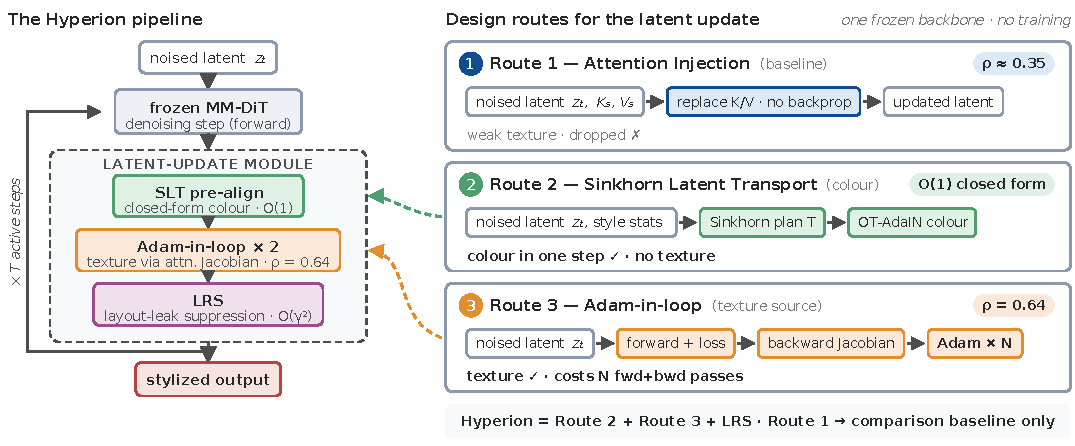
\includegraphics[width=\linewidth]{fig/figure/fig_framework_v3.pdf}
  \caption{%
    Design space of the method. \emph{Left} (dashed box = latent-update
    module): the final integrated
    \textbf{Hyperion pipeline}---at each active denoising step the frozen MM-DiT
    runs a style forward pass, SLT pre-aligns color in one closed-form step,
    two Adam steps inject cross-token texture through the self-attention
    Jacobian ($\rho{=}0.64$), and LRS suppresses layout leakage.
    \emph{Right}: the three latent-update design routes, each shown as a detailed
    module framework---\textbf{Route~1} Attention Injection (the training-free
    baseline that replaces content $K/V$ with style $K/V$ in one block, no
    backprop; $\rho{\approx}0.35$, weak texture); \textbf{Route~2}
    Sinkhorn Latent Transport (closed-form color alignment, $O(1)$, no
    texture); and \textbf{Route~3} Adam-in-loop (backprop through the frozen
    backbone, the source of spatial coherence, $\rho{=}0.64$). The Hyperion
    integrates Route~2 and Route~3 (with LRS layout suppression), discarding
    the injection baseline.%
  }
  \label{fig:architecture}
\end{figure*}

% ── Para 1: 鸿沟 ─────────────────────────────────────────────────────────────
Style transfer on modern image generation models falls into two
regimes that have so far remained largely separate.
\emph{Trained} methods (fine-tuned adapters, ControlNet-style
encoders~\cite{ipadapter2023,zhang2023controlnet,megastyle2026,xing2024csgo}) % 十修: remix2025 placeholder citation removed (unverifiable)
inject a style reference into the model's weights or cross-attention banks via
gradient descent, achieving high semantic fidelity and rich painterly texture.
\emph{Training-free} methods (attention $K/V$ injection, token
substitution, latent interpolation~%
\cite{hertz2024style,chung2024styleid,zhang2023inst,vshuffle2025,dualrf2025,xu2025stylessp,lin2025freecontrol})
require no optimization and generalize immediately to any reference image, but
their outputs exhibit only faint hue shifts with no discernible texture
structure, and their style fidelity—measured by the Contrastive Style
Descriptor (CSD)~\cite{somepalli2024measuring}—falls far below that of their
trained counterparts.
We argue that this gap originates from the underlying mechanism
rather than from model scale or training data (Sec.~\ref{sec:method:gap}).

% ── Para 2: 溯因 ─────────────────────────────────────────────────────────────
We investigate \emph{why} trained style methods produce coherent
texture while training-free ones do not, and attribute the difference to the
backpropagation graph.
It is well established that self-attention keys and values in diffusion
transformers encode both semantic content and fine-grained visual
texture~\cite{hertz2022prompt,chung2024styleid,seg4diff2025,gan2025ditf};
manipulating $K/V$ during denoising has therefore become the standard
mechanism for lightweight style injection~\cite{hertz2024style,xu2025stylessp}.
During fine-tuning, however, gradients flow back through the full diffusion
transformer and through its multi-head self-attention
Jacobian~\cite{vaswani2017attention}.
Neighboring tokens carry nearly identical keys—a structural consequence of
spatial continuity in the RoPE-encoded latent
grid~\cite{su2024rope,esser2024scaling}—so the rest of the image attends to
them with nearly equal weights; and because each token's output is a weighted
blend of value vectors, backpropagation through this \emph{value path}
therefore delivers nearly identical gradient signals to spatially adjacent
tokens, causing their latent updates to point in the same direction.
This spatial coherence is precisely what constitutes brushstroke texture:
it mirrors the long-range spatial correlations that Gatys
\etal~\cite{gatys2016image} identify as the defining statistical signature of
painterly style, now produced not by Gram-matrix optimization but as a natural
by-product of the attention Jacobian during backpropagation.
We make this claim precise in two ways: formally, by proving that
spatially smooth content keys force adjacent tokens to receive near-identical
gradient directions (Sec.~\ref{sec:method:gap},
Appendix~\ref{app:jacobian}); and empirically, by introducing the
\emph{spatial neighbor cosine}, a measure of how strongly adjacent per-token
updates align, under which backward-pass gradients prove far more spatially
coherent than any feedforward training-free update.
Training-free methods, because they perform no backward pass, lack this
cross-token coupling mechanism entirely.

% ── Para 3: 弥合 ─────────────────────────────────────────────────────────────
This observation suggests a direct remedy: \emph{introducing
backpropagation into the training-free setting}.
Starting from a standard inversion-interpolation baseline that blends content
and style attention features without any
optimization~\cite{hertz2024style,chung2024styleid,xu2025stylessp,avrahami2025stableflow},
we add an iterative Adam update~\cite{kingma2015adam} loop at each denoising
timestep.
At each step, a style forward pass extracts reference $K/V$ tensors; the
content latent is then updated by Adam on a style-alignment loss computed
from the content forward pass, with gradients flowing through the
self-attention Jacobian~\cite{vaswani2017attention}.
We call this \textbf{Adam-in-loop} style optimization.
To our knowledge, this is the first training-free pipeline on MM-DiT
whose outputs exhibit brushstroke texture, raising style fidelity from the
injection regime to a level comparable with trained adapters.

% ── Para 4: 速度瓶颈 ──────────────────────────────────────────────────────────
More iterations, however, mean slower generation: each Adam step costs a full
forward and backward pass through the model, and accumulated style pressure
gradually erodes faithfulness to the content
prompt~\cite{radford2021learning}.
Profiling the optimization reveals that the early iterations are
largely devoted to \emph{color distribution alignment}: the gradient is
dominated by a global low-frequency component that corrects bulk color
statistics, leaving only a small fraction of each step for the intended
texture signal.
Recent work confirms that high- and low-frequency components of diffusion
latents behave fundamentally differently during
generation~\cite{huang2025fresca,yuan2025consisid}, corroborating that a
single gradient step cannot serve both goals efficiently---a frequency
separation we later exploit directly through a frequency-domain Sinkhorn loss
(Sec.~\ref{sec:method:freq}).

% ── Para 5: OT 逼近 ──────────────────────────────────────────────────────────
This analysis reveals a mismatch between tool and task: gradient
descent is well suited to optimizing a differentiable objective through a
neural Jacobian, but poorly suited to global distribution alignment.
Color mismatch between the content and style latents is not a local,
high-curvature objective—it is a bulk statistical discrepancy between two
token populations~\cite{huang2017arbitrary}.
Optimal transport solves exactly this problem in closed form: it computes the
globally cost-minimizing assignment of content tokens to style tokens that
equates the two marginal
distributions~\cite{villani2009optimal,peyre2019computational,haviv2025wasserstein}.
Crucially, optimal transport does not pass through the attention Jacobian at
all—it operates directly in latent token space, bypassing the mechanism that
generates spatial coherence.
This property is precisely what is needed: optimal transport
resolves, in a single step, the sub-task that consumes most of Adam's
gradient budget, while leaving the Jacobian untouched for texture formation.
We implement this as \textbf{Sinkhorn Latent Transport (SLT)}, a soft
transport step driven by a doubly-stochastic Sinkhorn
plan~\cite{cuturi2013sinkhorn} whose marginal constraints guarantee that every
style token contributes to the result, preventing the mode collapse that
row-only softmax normalization permits~\cite{peyre2019computational}.
SLT matches color distributions at negligible cost; yet, used alone, its
outputs remain visually flat.
The reason is structural: the transport update at each token is independent of
every other token's update, so no mechanism couples adjacent positions, and
the spatially coherent structures that constitute brushstroke texture cannot
emerge (Sec.~\ref{sec:method:slt}).

% ── Para 6: Hyperion ───────────────────────────────────────────────────────────
The two mechanisms are complementary: SLT resolves what Adam
expends iterations on
(global color distribution via optimal
transport~\cite{villani2009optimal,haviv2025wasserstein}), while Adam produces
what SLT structurally cannot (cross-token gradient coupling via the
self-attention Jacobian~\cite{vaswani2017attention}).
Our \textbf{Hyperion} pipeline (Fig.~\ref{fig:architecture}) chains them within
each denoising step: SLT pre-aligns the color distribution, after which the
remaining Adam iterations are directed almost entirely toward texture.
We formalize this as a pre-alignment efficiency result
(Sec.~\ref{sec:method:hybrid}, Appendix~\ref{app:hybrid}) and confirm it
empirically: a Hyperion schedule with only two Adam iterations matches the
style fidelity of a far longer Adam-only schedule at a fraction of the
compute, and clearly outperforms Adam-only optimization at an equal compute
budget.

% ── Para 7: Contributions ─────────────────────────────────────────────────────
% 十一修 评阅#4: contribution 改 itemize、块内文献引用全部移除（各项均已在
% related work / method / experiments 相应位置引用）；随后的 Sec.2–7 路线图段
% 按老师意见删除。vaswani2017attention 在本节 Para 6 仍有引用，不失引。
\noindent\textbf{Contributions:}
\begin{itemize}[leftmargin=1.4em, itemsep=1pt, topsep=2pt]
  \item We identify the disparity between training-free and trained style
  transfer as a \emph{backpropagation gap}: trained methods derive spatial
  coherence from the self-attention Jacobian, whereas training-free injection
  methods lack this coupling entirely. We support this diagnosis with a formal
  coherence analysis and a reusable diagnostic, the \emph{spatial neighbor
  cosine} $\rho$, which we further extend to an output-image
  texture-coherence score (Sec.~\ref{sec:exp:texcoh}).
  \item We present \textbf{Hyperion}, a fully training-free style-transfer
  pipeline that bridges this gap by combining \textbf{Adam-in-loop} and
  \textbf{Sinkhorn Latent Transport (SLT)}. Adam-in-loop performs iterative
  backpropagation through a frozen MM-DiT at each denoising step, while SLT
  provides a closed-form optimal-transport color pre-alignment whose
  complementarity with Adam-in-loop is formally characterized.
  Frequency-domain Sinkhorn boosting and layout-residual suppression further
  enhance texture formation and suppress layout leakage.
  \item We validate Hyperion extensively on a 234-pair benchmark, where it
  raises CSD from $<0.15$ (injection) to $0.640$, exceeds an 8-iteration
  Adam-only schedule at $2.5\times$ lower forward-pass cost, outperforms four
  trained adapters on 19 of 21 style families, and extends effectively to
  image-to-image stylization. Controlled ablations further attribute the gains
  to the individual components.
\end{itemize}
